% Fig. 3.7 -- 非積空間的聯合值域如何把平面分區，與 Fig. 3.6 的九宮格對照。
% 書稿來源: mathstatch3.tex 第 814 行的 tikzpicture (scale=1.3)。
%
% 幾何一律照書稿: 三角形值域 0 <= x <= y <= 1、邊界 x = y 的斜線、
% 橫線 y = 1、縱線 x = 1 只在三角形所佔的高度之外出現，四個非零區塊
% 各標一個積分式，x < 0 的左行與 y < 0 的下列共五處標 0。
%
% 對書稿的四處調整:
%   1. 書稿的縱線 x = 1 下段畫滿一整格，本圖收成座標軸下的一小段，只作標號之用。
%   2. 書稿的四個積分式壓在斜線與縱軸之上，本圖把三角形放大並重排標示位置，
%      各標示與線條之間至少留 0.18cm。
%   3. 填色由 gray 0.2 改為 journalaccent 0.15。
%   4. 字級: 書稿的 $f_{\sssig XY}$ 走 scriptscriptstyle，在 350px 顯示寬之下
%      下標不到 7px。此處改為一般下標，全圖走 10pt，並以 \DeclareMathSizes
%      把 script 級撐到 9pt，最小字因而是 9pt。
%
% 量測: viewBox 寬 269.383pt，350px 之下放大 1.2993 倍，最小字 9pt 折合 11.69px。
%
% 產製:
%   pdflatex non-product-space-regions.tex
%   pdftocairo -svg non-product-space-regions.pdf ../../images/teaching-topics/non-product-space-regions.svg

\documentclass[tikz,border=2pt]{standalone}
\usepackage{amsmath}
\usepackage{amssymb}
\usepackage{xcolor}

\definecolor{journalink}{HTML}{1F1C18}
\definecolor{journalmuted}{HTML}{8A7F72}
\definecolor{journalaccent}{HTML}{9C2D2D}

%% 下標與積分上下限一律撐到 9pt。
\DeclareMathSizes{10}{10}{9}{9}

\begin{document}
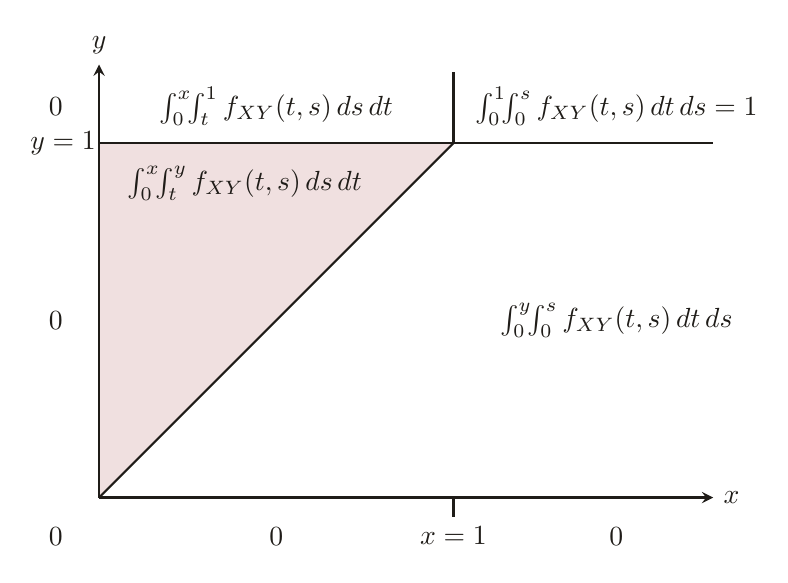
\begin{tikzpicture}[x=1cm, y=1cm, >=stealth,
                    every node/.style={journalink, font=\normalsize},
                    intg/.style={journalink, inner sep=1pt}]

  %% 聯合值域 0 <= x <= y <= 1 所對應的三角形
  \fill[journalaccent, fill opacity=0.15] (1,1) -- (5.5,5.5) -- (1,5.5) -- cycle;

  %% 值域的斜邊界 x = y
  \draw[journalink, line width=0.8pt] (1,1) -- (5.5,5.5);

  %% 上邊界 y = 1
  \draw[journalink, line width=0.8pt] (1,5.5) -- (8.8,5.5);
  \node[journalink, left, inner sep=1pt] at (1,5.5) {$y=1$};

  %% 邊界 x = 1: 只有在 y > 1 之處才是分區的界線，
  %% 故上段畫實線，座標軸下另留一小段標號。
  \draw[journalink, line width=0.8pt] (5.5,5.5) -- (5.5,6.4);
  \draw[journalink, line width=0.8pt] (5.5,1) -- (5.5,0.75);
  \node[journalink, below] at (5.5,0.75) {$x=1$};

  %% 座標軸
  \draw[journalink, line width=0.8pt, ->] (1,1) -- (8.8,1) node[right] {$x$};
  \draw[journalink, line width=0.8pt, ->] (1,1) -- (1,6.5) node[above] {$y$};

  %% 四個非零區塊各自的積分寫法
  \node[intg] at (2.85,4.99)
    {$\int_{0}^{x}\!\!\int_{t}^{y} f_{XY}(t,s)\,ds\,dt$};
  \node[intg] at (7.57,3.25)
    {$\int_{0}^{y}\!\!\int_{0}^{s} f_{XY}(t,s)\,dt\,ds$};
  \node[intg] at (3.25,5.97)
    {$\int_{0}^{x}\!\!\int_{t}^{1} f_{XY}(t,s)\,ds\,dt$};
  \node[intg] at (7.57,5.97)
    {$\int_{0}^{1}\!\!\int_{0}^{s} f_{XY}(t,s)\,dt\,ds=1$};

  %% 其餘各區塊的 cdf 值皆為 0
  \node at (0.45,5.97) {$0$};
  \node at (0.45,3.25) {$0$};
  \node at (0.45,0.50) {$0$};
  \node at (3.25,0.50) {$0$};
  \node at (7.57,0.50) {$0$};

\end{tikzpicture}
\end{document}
